\chapter{An\'alisis del Sistema}
\section{Requerimientos Funcionales}
\begin{indentar}
De manera general, los requerimientos que se han pedido para mejorar el Portal son los siguientes:
\begin{itemize}
\item A\~nadir el m\'odulo de pago en l\'inea;
\item Dar soporte para varios idiomas;
\item Mostrar res\'umenes de evaluaciones, con los siguientes datos: recomendaci\'on y exportaci\'on de los datos ingresados por los evaluadores;
\item Implementar requerimientos adicionales pedidos por el Sub - Componente de Telecomunicaciones, tales como:
	\begin{itemize}
	\item Manejar copias ocultas para emails de rechazo de art\'iculos, es decir, el correo electr\'onico debe enviarse con copia al correo electr\'onico del evento y con copia oculta al administrador que rechaza el art\'iculo;
	\item Mayor flexibilidad en el momento de la elaboraci\'on y modificaci\'on de las preguntas frecuentes;
	\item Agregar la posibilidad de subir un resumen previo -por parte del usuario participante del evento cient\'ifico- al art\'iculo cient\'ifico final  que se va a evaluar;
	\item Se debe poder modificar un art\'iculo sin tener que borrar y volverlo a subir;
	\item Despu\'es de evaluado un art\'iculo, se debe seguir mostrando -a los administradores del evento- quienes fueron sus evaluadores;
	\item El registro del usuario debe ser internacional y no s\'olo dirigido a nuestro pa\'is;
	\item Corregir lo siguiente: un autor no debe poder evaluar su propio art\'iculo, los autores secundarios tambi\'en deben constar en la lista de un art\'iculo, y en el manejo de sesiones (a veces se sale del sistema y se desea ingresar con clave err\'onea, el sistema lo permite);
	\item Generar los siguientes reportes: trabajos por autores, evaluadores asignados a cada art\'iculo, res\'umenes de art\'iculos clasificados con su respectiva nota y el estado de cada art\'iculo. Exportar los reportes a los formatos: CSV y pdf;
	\item Adjuntar los art\'iculos de derecho de traspaso de los art\'iculos aceptados;
	\item Permitir que el administrador pueda eliminar un art\'iculo;
	\item Ocultar clave de la lista de los usuarios;
	\item Manejar un email de contacto para cada evento diferente;
	\item Guardar la fecha de publicaci\'on de un art\'iculo, cuando se lo suba al Sistema;
	\item En los registros: cuando un usuario realice un pago en efectivo, permitir ingresar el valor que pag\'o; en el pre registro notificar al usuario la fecha l\'imite para realizar el pago correspondiente;
	\item Poder escoger el autor de un paper en caso de que una persona alterna suba el art\'iculo por el autor.
	\end{itemize}
\end{itemize}
\end{indentar}

\section{Requerimientos No Funcionales}
Los requerimientos no funcionales que se desea para el Portal son los siguientes:
\begin{indentar}
\begin{itemize}
\item Manejo m\'as apropiado de IHM\footnote{Interacci\'on Hombre - M\'aquina.}: estandarizaci\'on de los \'iconos de la aplicaci\'on y mostrar errores espec\'ificos, no generales. (Mejor retroalimentaci\'on);
\item Utilizar MVC 2 en el dise\~no e implementaci\'on; puesto que este ofrece mayor flexibilidad al producto final;
\item Reparar defectos encontrados, entre los cuales existen algunos que afectan al rendimiento de la Aplicaci\'on Web, tales como: la optimizaci\'on de las consultas a la Base de Datos;
\item Separar la parte de manejo de eventos para que pueda instalarse y ejecutarse independientemente de la parte de administraci\'on de grupos de investigaci\'on y sus \'areas de trabajo.
\end{itemize}
Los requerimientos m\'inimos, en cuanto a hardware, son los siguientes:
\begin{itemize}
\item Capacidad de memoria en el servidor: para un buen desempe\~no del sistema, una memoria de 2 GB de RAM \'o superior.
\item Capacidad de disco duro en el servidor: se recomienda un disco duro de 80 GB como m\'inimo.
\item Tipo de procesador en el servidor: Se recomienda un procesador Core 2 Duo 2.0GHz.
\item Ancho de Banda para el servidor: Ancho de Banda recomendado 128 Mbits.
\item Navegadores: Para un buen uso del sistema se recomienda Firefox 3.0 \'o superior.
\item Sistema Operativo en el Servidor: Microsoft Windows XP \'o superior, o cualquier distribuci\'on de GNU/Linux, se recomienda Ubuntu.
\end{itemize}
\end{indentar}

\section{Especificaci\'on del Modelo Independiente de la Plataforma (PIM) usando t\'ecnicas de MERODE}
\begin{indentar}
MERODE nos permite la posibilidad de modelar el dominio de manera independiente de la plataforma que se desee implementar en un futuro pr\'oximo, en nuestro caso deseamos diagramar un PIM (Platform Independent Model) mediante un EDG, fue dise\~nado mediante la herramienta llamada MERMAID\footnote{\url{http://merode.econ.kuleuven.ac.be/activate.aspx}}.

Es necesario mencionar, el hecho de haber diagramado en un solo PIM el dominio de la administraci\'on de usuarios, la administraci\'on de eventos, la convocatoria y la evaluaci\'on de art\'iculos. Al realizar esta actividad de revisi\'on y redise\~no, se ha pensado de manera sistem\'atica la diagramaci\'on de un solo PIM en varios m\'odulos.
\end{indentar}

\subsection{El gr\'afico de la dependencia de existencia (EDG)}
\begin{indentar}
A continuaci\'on se muestran los Gr\'aficos de la Dependencia de existencia o EDG, como sistema (\ref{edg:websae}) y luego separado por m\'odulos para un mejor estudio de ellos.

\begin{landscape}
\begin{figure}
  \centering
    {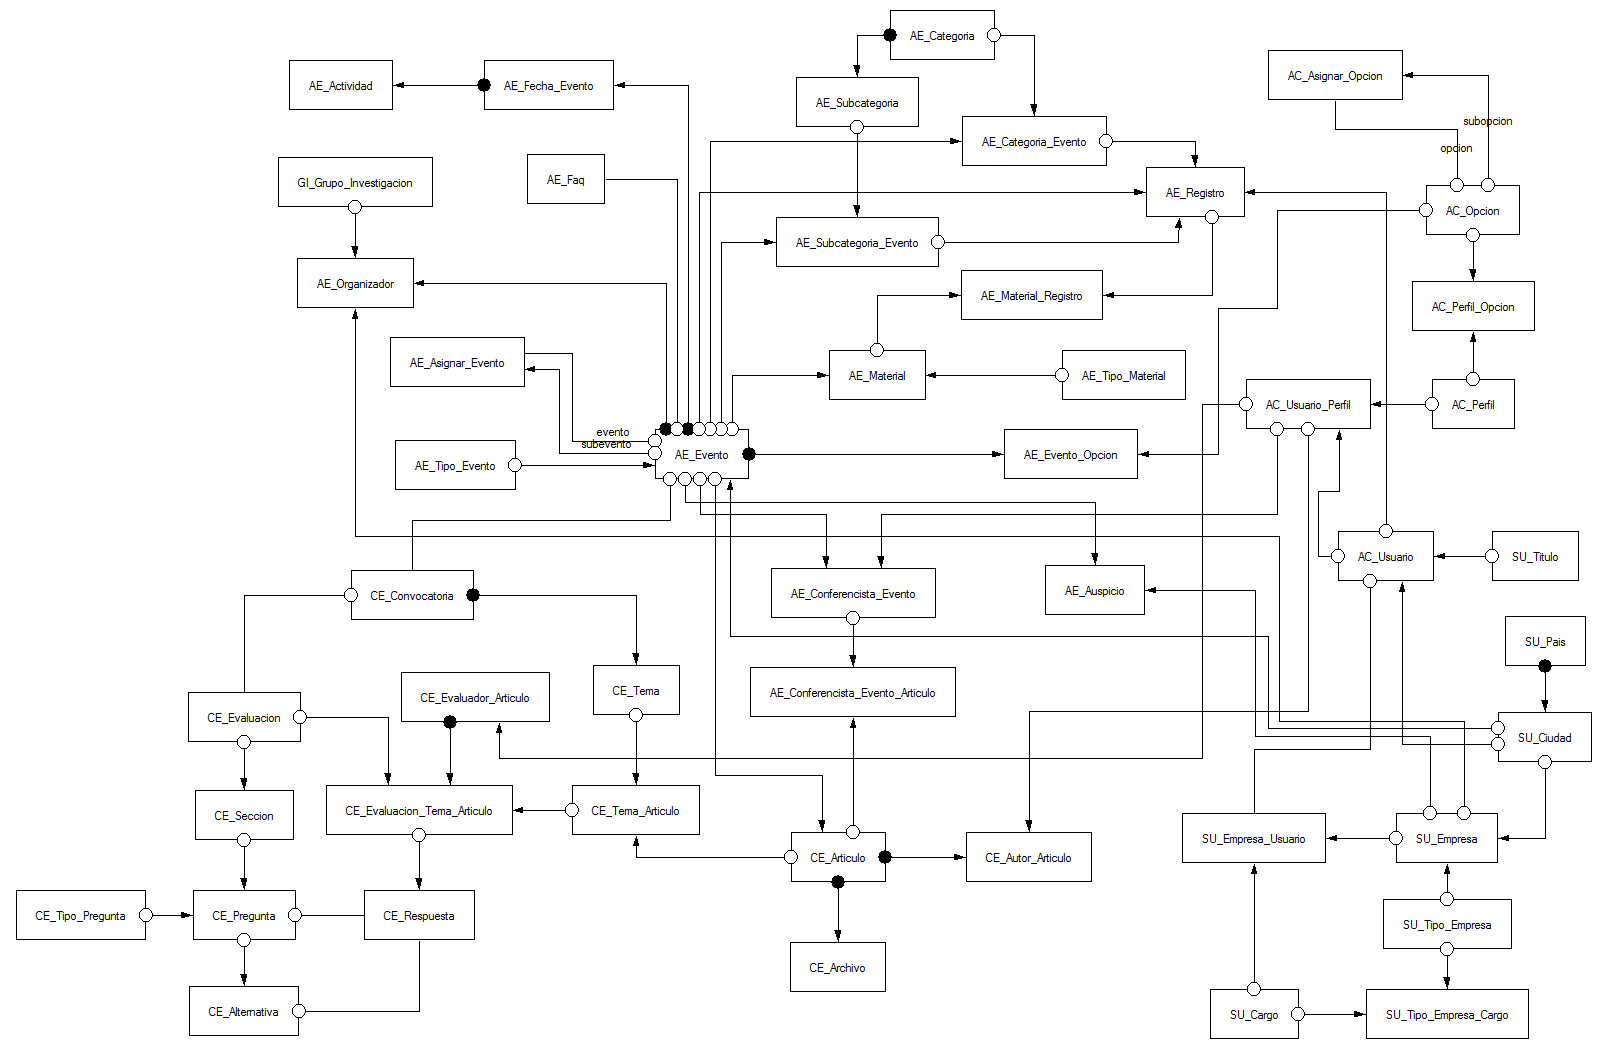
\includegraphics[width=1.5\textwidth]{images/merode-websae.eps}}
  \caption{EDG - Sistema Web para la Administraci\'on de Eventos Cient\'ificos (WebSAE)}
  \label{edg:websae}
\end{figure}
\end{landscape}

Se necesitaron un total de 48 objetos para implementar el Sistema actual, que ha sido denominado como \textbf{WebSAE}. En el Sistema original, denominado como \textbf{AppVlir8}, se dise\~n\'o con 42 objetos en total, es decir, que en el actual se han aumentado 6 objetos.

A continuaci\'on se enumerar\'an los objetos propios de cada m\'odulo con el correspondiente EDG:

\textbf{M\'ODULO DE ADMINISTRACI\'ON CENTRAL (MAC)}

\textbf{MAC} (\ref{edg:mac}) tiene 6 objetos que se listar\'an a continuaci\'on:

\begin{enumerate}
\item AC\_Usuario
\item AC\_Usuario\_Perfil
\item AC\_Perfil
\item AC\_Perfil\_Opcion
\item AC\_Opcion
\item AC\_Asignar\_Opcion
\end{enumerate}

Es necesario enfatizar que \textbf{MAC} surge en el momento de pensar en la Arquitectura de \textbf{WebSAE}, la mitad  de los objetos son nuevos, a continuaci\'on la siguiente ~\ref{diferencias:websae-appvlir8-mac} nos explica las diferencias entre los objetos, dependiendo si es el Sistema actual o el anterior.

\begin{table}
	\begin{center}
	\begin{tabular}{|p{1.5in}|p{1.5in}|p{1.8in}|}
		\hline
		\textbf{WebSAE} & \textbf{AppVlir8} & \textbf{Observaciones} \\
		\hline\hline
		  AC\_Usuario\_Perfil	& Rol\_Usuario &  \\
		\hline
		  AC\_Perfil				& Rol		 		&  \\
		\hline
		  AC\_Perfil\_Opcion		& Menu	 		& Objeto que asigna las opciones, dependiendo del perfil que se haya deseado crear. \\
		\hline
		  AC\_Opcion				& Opcion\_Menu	& Son las diversas opciones que se le presentan al usuario, dependiendo del perfil que tenga asignado.  \\
		\hline
		  AC\_Asignar\_Opcion	& Submenu 		& Este objeto nos sirve para manejar la recursi\'on entre las opciones, debido a que normalmente existen subopciones entre las opciones\footnote{\textbf{MERODE} no permite dise\~nar recursividad en un mismo objeto, por eso la necesidad de crear otro objeto que maneje este tipo de especificaciones.}. \\
		\hline
	\end{tabular}
	\caption{Diferencias entre los objetos de \textbf{WebSAE} y \textbf{AppVlir8}, en \textbf{MAC}.}\label{diferencias:websae-appvlir8-mac}
	\end{center}
\end{table}

\begin{figure}
  \centering
    {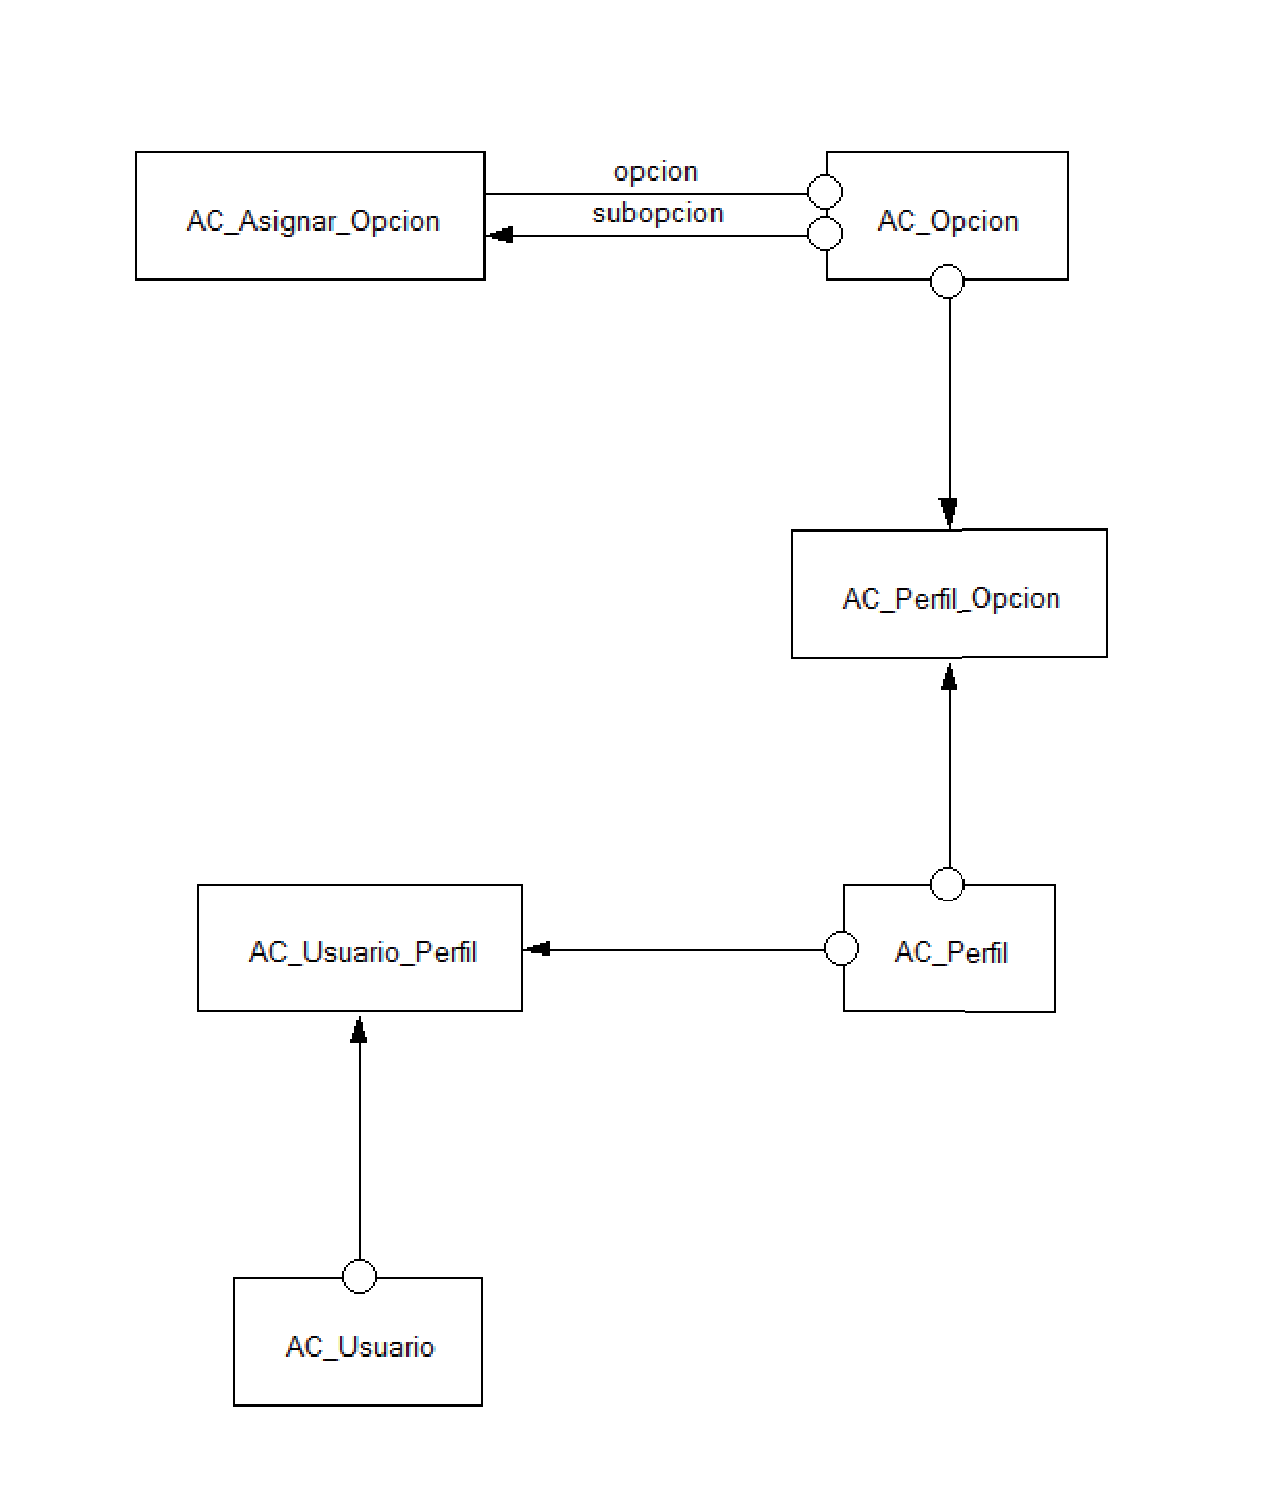
\includegraphics[width=0.5\textwidth]{images/merode-mac.eps}}
  \caption{EDG - M\'odulo de Administraci\'on Central (MAC)}
  \label{edg:mac}
\end{figure}

\textbf{M\'ODULO DE SUSCRIPCI\'ON DE USUARIOS (MSU)}

\textbf{MSU} (\ref{edg:msu}) tiene 8 objetos que se listar\'an a continuaci\'on:

\begin{enumerate}
\item SU\_Titulo
\item SU\_Pais
\item SU\_Ciudad
\item SU\_Empresa
\item SU\_Tipo\_Empresa
\item SU\_Empresa\_Usuario
\item SU\_Tipo\_Empresa\_Cargo
\item SU\_Cargo
\end{enumerate}

En la siguiente ~\ref{diferencias:websae-appvlir8-msu} nos explica las diferencias entre los objetos, dependiendo si es el Sistema actual o el anterior.

\begin{table}
	\begin{center}
	\begin{tabular}{|l|l|p{1.5in}|}
		\hline
		\textbf{WebSAE} & \textbf{AppVlir8} & \textbf{Observaciones} \\
		\hline\hline
		  	SU\_Tipo\_Empresa\_Cargo	&  & Este objeto surgi\'o debido a que anteriormente Cargo depend\'ia de manera directa de Tipo\_Empresa, en la revisi\'on del dise\~no se cambi\'o esa relaci\'on agregando un objeto, de tal manera que ahora Cargo y Tipo de Empresa son independientes. \\
		\hline
	\end{tabular}
	\caption{Diferencias entre los objetos de \textbf{WebSAE} y \textbf{AppVlir8}, en \textbf{MSU}.}\label{diferencias:websae-appvlir8-msu}
	\end{center}
\end{table}

\begin{figure}
  \centering
    {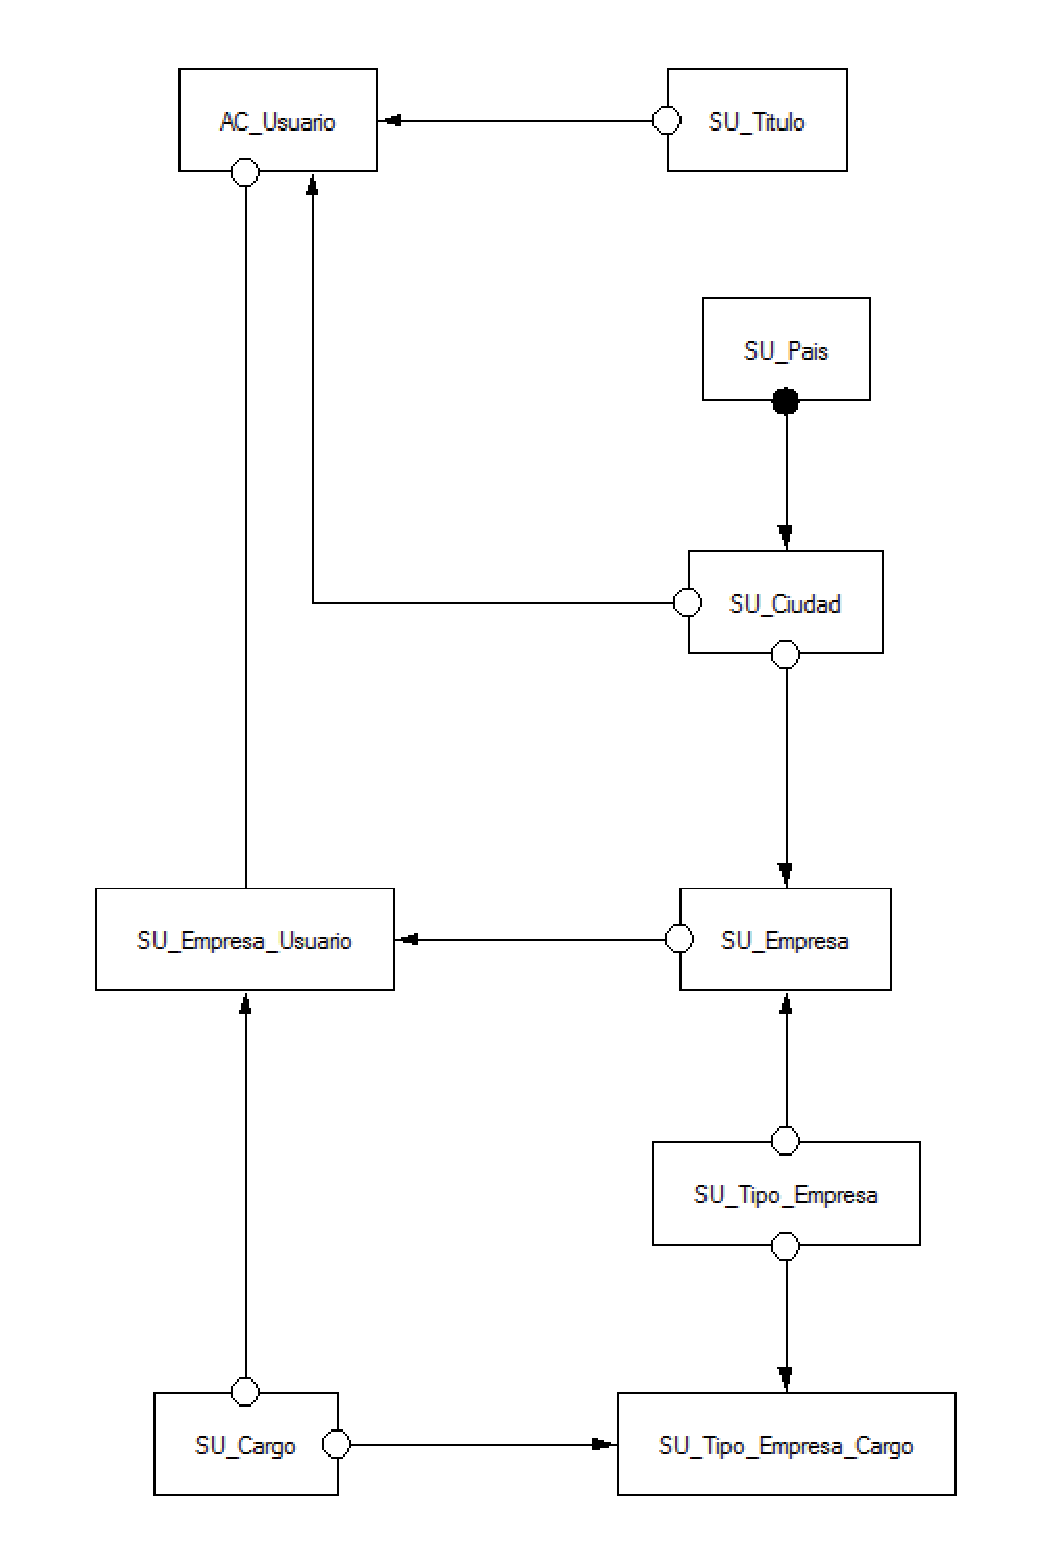
\includegraphics[width=0.5\textwidth]{images/merode-msu.eps}}
  \caption{EDG - M\'odulo de Suscripci\'on de Usuarios (MSU)}
  \label{edg:msu}
\end{figure}

\textbf{M\'ODULO DE ADMINISTRACI\'ON DE EVENTOS (MAE)}

\textbf{MAE} (\ref{edg:mae}) tiene 19 objetos que se listar\'an a continuaci\'on:

\begin{enumerate}
\item AE\_Actividad
\item AE\_Asignar\_Evento
\item AE\_Auspicio
\item AE\_Categoria
\item AE\_Categoria\_Evento
\item AE\_Conferencista\_Evento
\item AE\_Conferencista\_Evento\_Articulo
\item AE\_Evento
\item AE\_Evento\_Opcion
\item AE\_Faq
\item AE\_Fecha\_Evento
\item AE\_Material
\item AE\_Material\_Registro
\item AE\_Organizador
\item AE\_Registro
\item AE\_Subcategoria
\item AE\_Subcategoria\_Evento
\item AE\_Tipo\_Evento
\item AE\_Tipo\_Material
\end{enumerate}

En la siguiente ~\ref{diferencias:websae-appvlir8-mae} nos explica las diferencias entre los objetos, dependiendo si es el Sistema actual o el anterior.

\begin{table}
	\begin{center}
	\begin{tabular}{|p{1.5in}|p{1.5in}|p{1.8in}|}
		\hline
		\textbf{WebSAE} & \textbf{AppVlir8} & \textbf{Observaciones} \\
		\hline\hline
			AE\_Asignar\_Evento & Subevento\_Evento &  \\
		\hline
		  	AE\_Auspicio 		& Auspicio & Adem\'as de la relaci\'on existente con una Empresa, tambi\'en se le agreg\'o la relaci\'on con un Grupo de Investigaci\'on, debido a que tambi\'en pueden ser auspiciantes sin ser los Organizadores. \\
		\hline
		  	AE\_Categoria\_ Evento		& Categoria\_Evento & Es el precio dependiendo de la Categor\'ia. \\
		\hline
		  	AE\_Subcategoria\_ Evento	& Subcategoria\_Evento & Es el porcentaje dependiendo de la Subcategor\'ia. \\
		\hline
		  	AE\_Conferencista\_ Evento	& Conferencista\_Evento & Este objeto en el anterior Sistema estaba en \textbf{MCE}, pero debido a que muchas veces existen conferencistas que son invitados y no necesariamente entran en el proceso de evaluaci\'on de art\'iculos, de ah\'i en la necesidad de cambiar de m\'odulo a este objeto. \\
		\hline
		  	AE\_Conferencista\_ Evento\_Articulo	& AE\_Conferencista\_ Articulo &  \\
		\hline
		  	AE\_Evento\_Opcion						& Menu\_Evento &  \\
		\hline
		  	 & Pregunta\_Faq & Eliminado de WebSAE, debido a que en el objeto Faq, se guardan las preguntas en HTML. \\
		\hline
		  	 & Respuesta\_Faq & Eliminado de WebSAE, por la raz\'on anterior. \\
		\hline
		  	 & Correo & Eliminado de WebSAE. \\
		\hline
	\end{tabular}
	\caption{Diferencias entre los objetos de \textbf{WebSAE} y \textbf{AppVlir8}, en \textbf{MAE}.}\label{diferencias:websae-appvlir8-mae}
	\end{center}
\end{table}

\begin{landscape}
\begin{figure}
  \centering
    {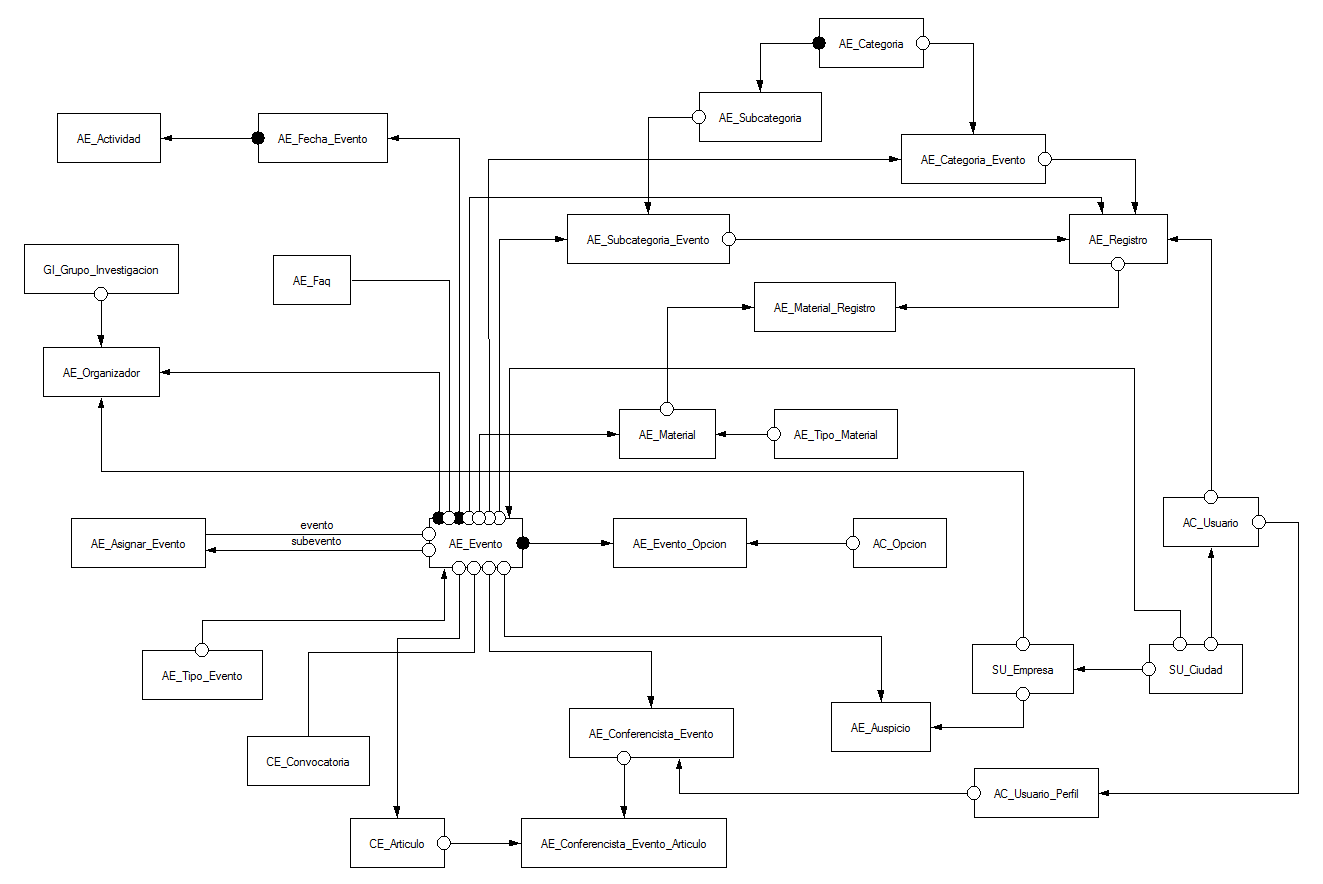
\includegraphics[width=1.1\textwidth]{images/merode-mae.eps}}
  \caption{EDG - M\'odulo de Administraci\'on de Eventos (MAE)}
  \label{edg:mae}
\end{figure}
\end{landscape}

\textbf{M\'ODULO DE CONVOCATORIA Y EVALUACI\'ON DE ART\'ICULOS (MCE)}

\textbf{MCE} (\ref{edg:mce}) tiene 14 objetos que se listar\'an a continuaci\'on:

\begin{enumerate}
\item CE\_Alternativa
\item CE\_Archivo
\item CE\_Articulo
\item CE\_Autor\_Articulo
\item CE\_Convocatoria
\item CE\_Evaluacion
\item CE\_Evaluacion\_Tema\_Articulo
\item CE\_Evaluador\_Articulo
\item CE\_Pregunta
\item CE\_Respuesta
\item CE\_Seccion
\item CE\_Tema
\item CE\_Tema\_Articulo
\item CE\_Tipo\_Pregunta
\end{enumerate}

En la siguiente ~\ref{diferencias:websae-appvlir8-mce} nos explica las diferencias entre los objetos, dependiendo si es el Sistema actual o el anterior.

\begin{table}
	\begin{center}
	\begin{tabular}{|p{1.5in}|p{1.5in}|p{1.8in}|}
		\hline
		\textbf{WebSAE} & \textbf{AppVlir8} & \textbf{Observaciones} \\
		\hline\hline
			CE\_Archivo &  & Agregado debido a que se desea tener todos los archivos que se generen en el proceso de la evaluaci\'on por cada usuario que haya subido su art\'iculo para participar de la convocatoria. \\
		\hline
			CE\_Respuesta & Respuestas & \\
		\hline
			 & Articulo\_Evento & Eliminado de WebSAE, se incluy\'o una relaci\'on directa entre CE\_Evento y CE\_Articulo, en el que CE\_Articulo depende de CE\_Evento. \\
		\hline
	\end{tabular}
	\caption{Diferencias entre los objetos de \textbf{WebSAE} y \textbf{AppVlir8}, en \textbf{MCE}.}\label{diferencias:websae-appvlir8-mce}
	\end{center}
\end{table}

\begin{landscape}
\begin{figure}
  \centering
    {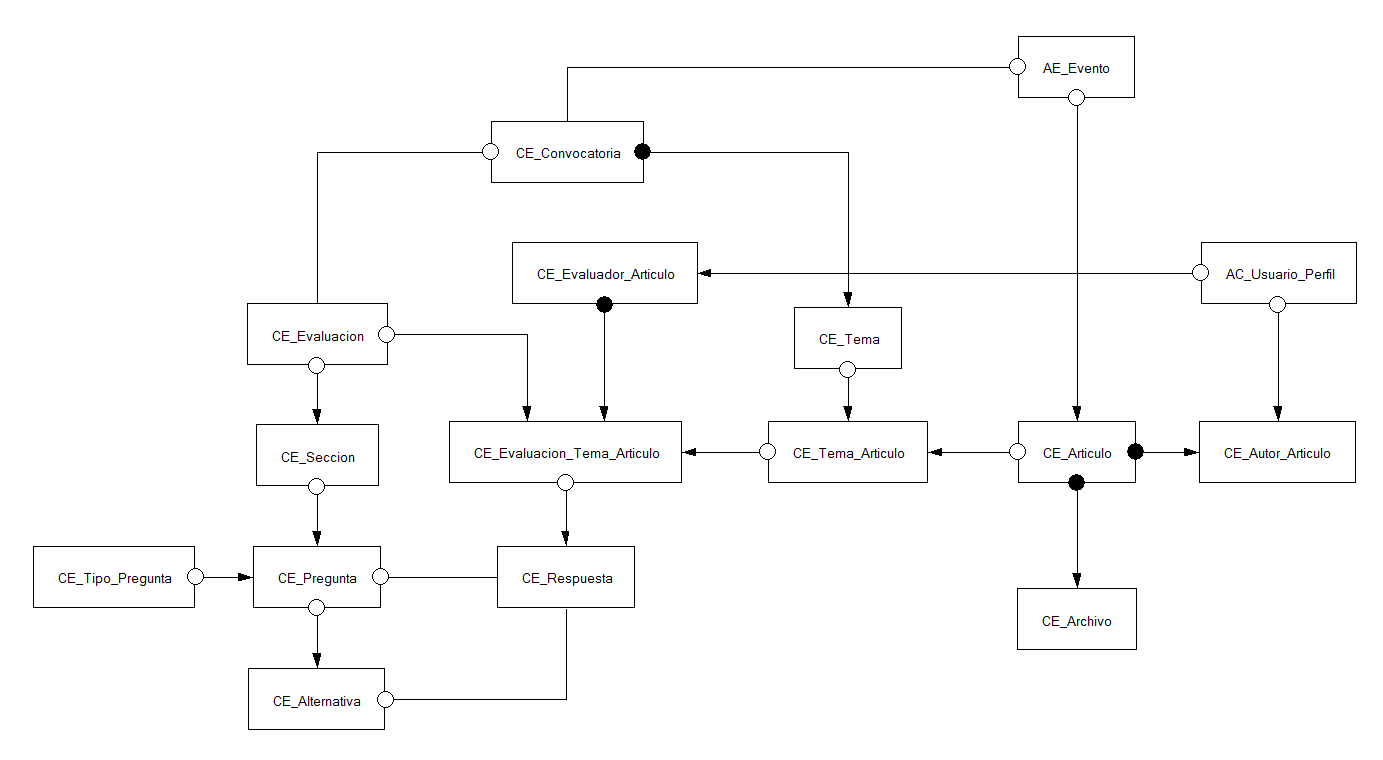
\includegraphics[width=1.3\textwidth]{images/merode-mce.eps}}
  \caption{EDG - M\'odulo de Convocatoria y Evaluaci\'on de Art\'iculos (MCE)}
  \label{edg:mce}
\end{figure}
\end{landscape}
\end{indentar}

\subsection{La tabla de eventos de objetos (OET)}
\begin{indentar}
Para presentar la Tabla de Objetos de Eventos\footnote{Es una matriz que contiene una fila por cada tipo de evento y una columna por cada tipo de objeto, como se ha detallado en el cap\'itulo 2.}, se ha considerado separarla por objetos para que pueda ser apreciada de una mejor manera.

\begin{table}
	\begin{center}
	\begin{tabular}{|r|c|}
		\hline
				& \textbf{AE\_Evento} \\
		\hline\hline
			registrar\_evento	& O/C \\
		\hline
			modificar\_evento	& O/M \\
		\hline
			eliminar\_evento	& O/E \\
		\hline
			registrar\_material	& A/M \\
		\hline
			modificar\_material	& A/M \\
		\hline
			eliminar\_material	& A/M \\
		\hline
			registrar\_material\_subevento	& A/M \\
		\hline
			modificar\_material\_subevento	& A/M \\
		\hline
			eliminar\_material\_subevento	& A/M \\
		\hline
			asignar\_evento\_opcion	& A/M \\
		\hline
			actualizar\_faq	& A/M \\
		\hline
			registrar\_agenda	& A/M \\
		\hline
			modificar\_agenda	& A/M \\
		\hline
			eliminar\_agenda	& A/M \\
		\hline
			registrar\_auspiciante	& A/M \\
		\hline
			modificar\_auspiciante	& A/M \\
		\hline
			eliminar\_auspiciante	& A/M \\
		\hline
			registrar\_horario	& A/M \\
		\hline
			modificar\_horario	& A/M \\
		\hline
			eliminar\_horario	& A/M \\
		\hline
			registrar\_subcategoria	& A/M \\
		\hline
			modificar\_subcategoria	& A/M \\
		\hline
			eliminar\_subcategoria	& A/M \\
		\hline
			registrar\_subcategoria\_evento	& A/M \\
		\hline
			modificar\_subcategoria\_evento	& A/M \\
		\hline
			eliminar\_subcategoria\_evento	& A/M \\
		\hline
			registrar\_subcategoria\_subevento	& A/M \\
		\hline
			modificar\_subcategoria\_subevento	& A/M \\
		\hline
			eliminar\_subcategoria\_subevento	& A/M \\
		\hline
			registrar\_categoria\_evento	& A/M \\
		\hline
			modificar\_categoria\_evento	& A/M \\
		\hline
			eliminar\_categoria\_evento	& A/M \\
		\hline
			registrar\_categoria\_subevento	& A/M \\
		\hline
			modificar\_categoria\_subevento	& A/M \\
		\hline
			eliminar\_categoria\_subevento	& A/M \\
		\hline
			registrar\_conferencista\_evento	& A/M \\
		\hline
			modificar\_conferencista\_evento	& A/M \\
		\hline
			eliminar\_conferencista\_evento	& A/M \\
		\hline
			registrar\_conferencista\_subevento	& A/M \\
		\hline
			modificar\_conferencista\_subevento	& A/M \\
		\hline
			eliminar\_conferencista\_subevento	& A/M \\
		\hline
	\end{tabular}
	\caption{OET - Objeto AE\_Evento (Parte 1)}
	\label{oet:evento}
	\end{center}
\end{table}

\begin{table}
	\begin{center}
	\begin{tabular}{|r|c|}
		\hline
				& \textbf{AE\_Evento} \\
		\hline\hline
			registrar\_organizador	& A/M \\
		\hline
			eliminar\_organizador	& A/M \\
		\hline
			registrar\_subevento	& O/C \\
		\hline
			modificar\_subevento	& O/M \\
		\hline
			eliminar\_subevento	& O/E \\
		\hline
			registrar\_usuario\_evento	& A/M \\
		\hline
			eliminar\_usuario\_evento	& A/M \\
		\hline
	\end{tabular}
	\caption{OET - Objeto AE\_Evento (Parte 2)}
	\label{oet:evento}
	\end{center}
\end{table}

\end{indentar}

\subsection{M\'aquina de estados finitos relevantes (FSM)}
\begin{indentar}

\begin{figure}
  \centering
    {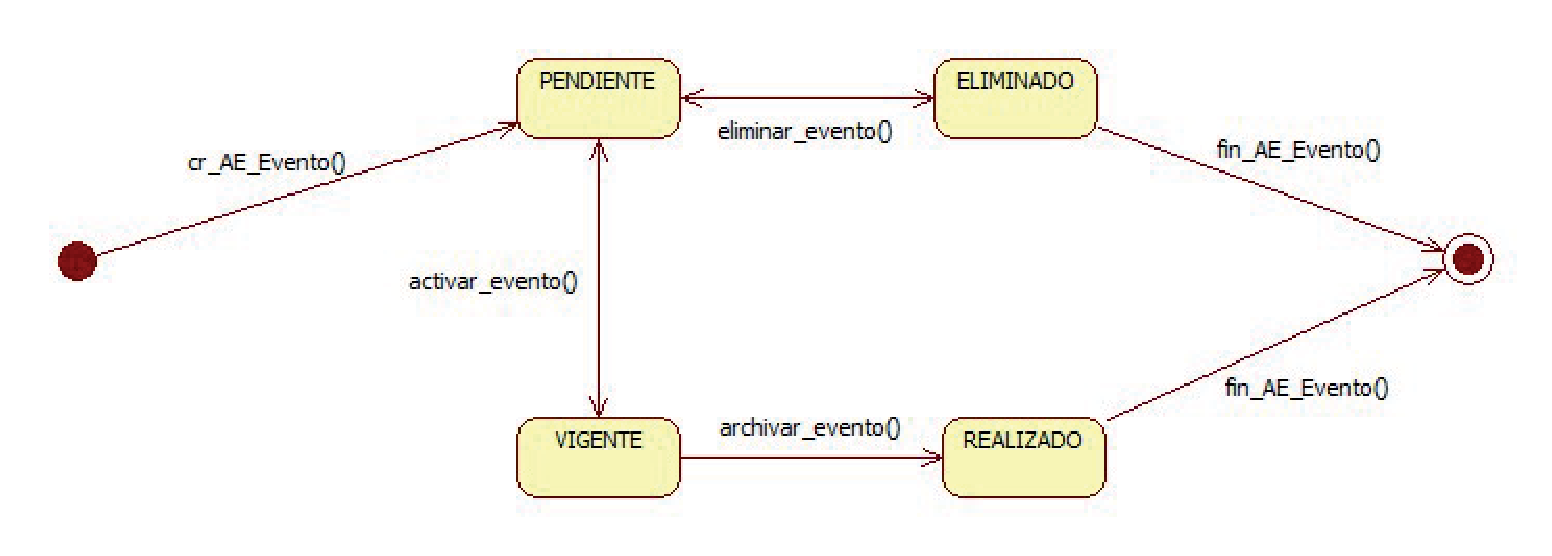
\includegraphics[width=1.0\textwidth]{images/estado-evento.eps}}
  \caption{FSM - Estados del Objeto AE\_Evento}
  \label{estados:ae_evento}
\end{figure}

\begin{figure}
  \centering
    {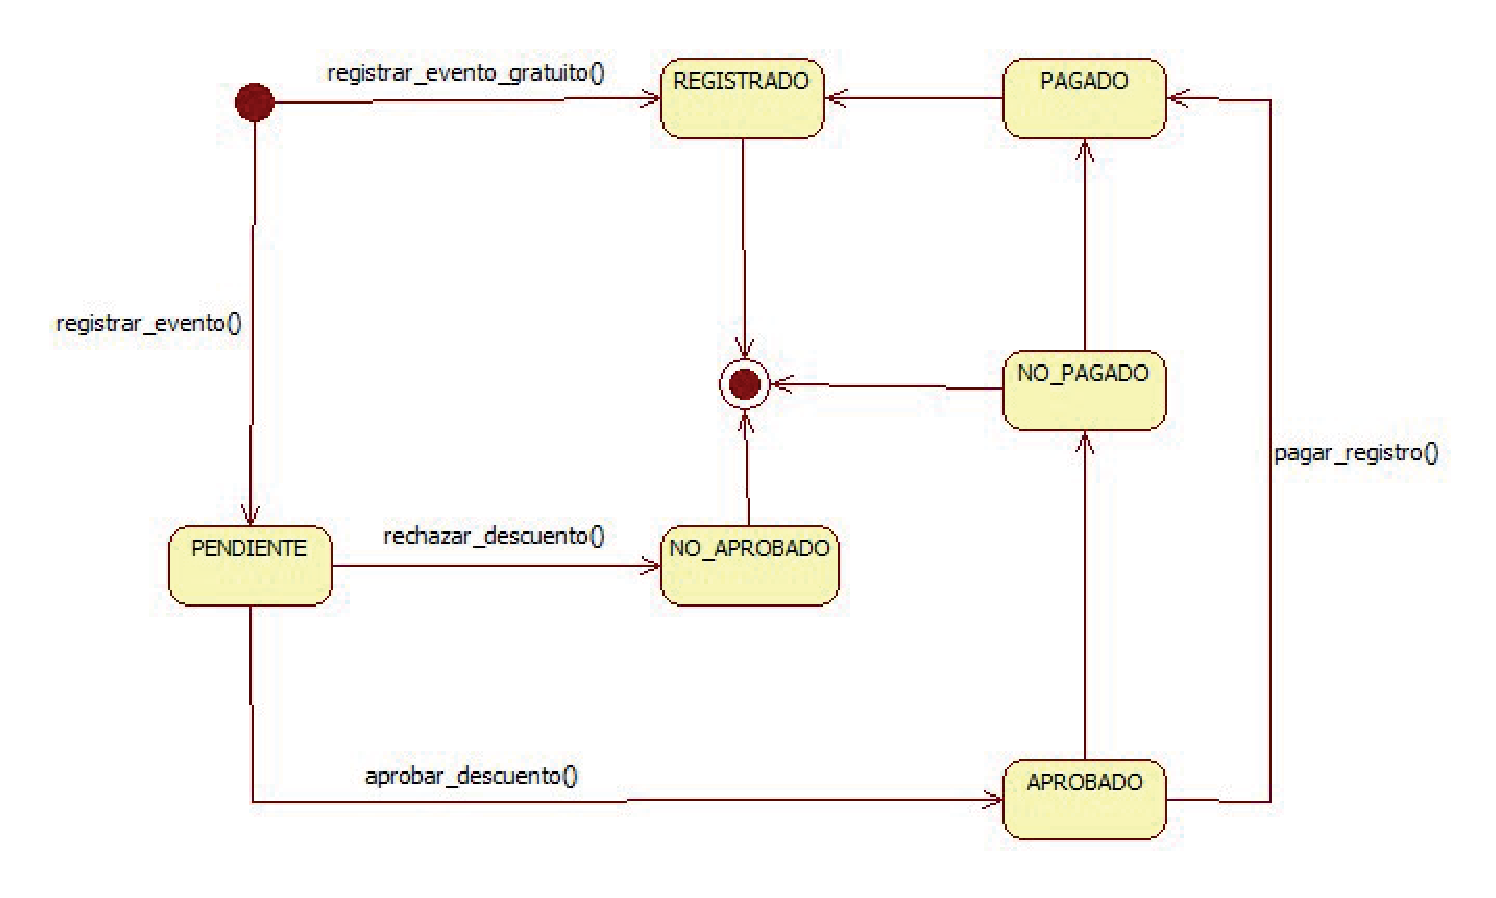
\includegraphics[width=1.0\textwidth]{images/estado-registro.eps}}
  \caption{FSM - Estados del Objeto AE\_Registro}
  \label{estados:ae_registro}
\end{figure}

\end{indentar}

\section{Definici\'on del Modelo espec\'ifico de la plataforma (PSM)}
\begin{indentar}
Luego de elaborar el correspondiente EDG, se pas\'o a la etapa del PSM, el cual fue diagramado mediante una herramienta Open Source, llamada StarUML\footnote{\url{http://staruml.sourceforge.net/en/}}.

Los m\'odulos del PIM anterior tan s\'olo fueron pasados al simil en UML, para su correspondiente transformaci\'on al c\'odigo, en el momento debido.
\begin{landscape}
\begin{figure}
  \centering
    {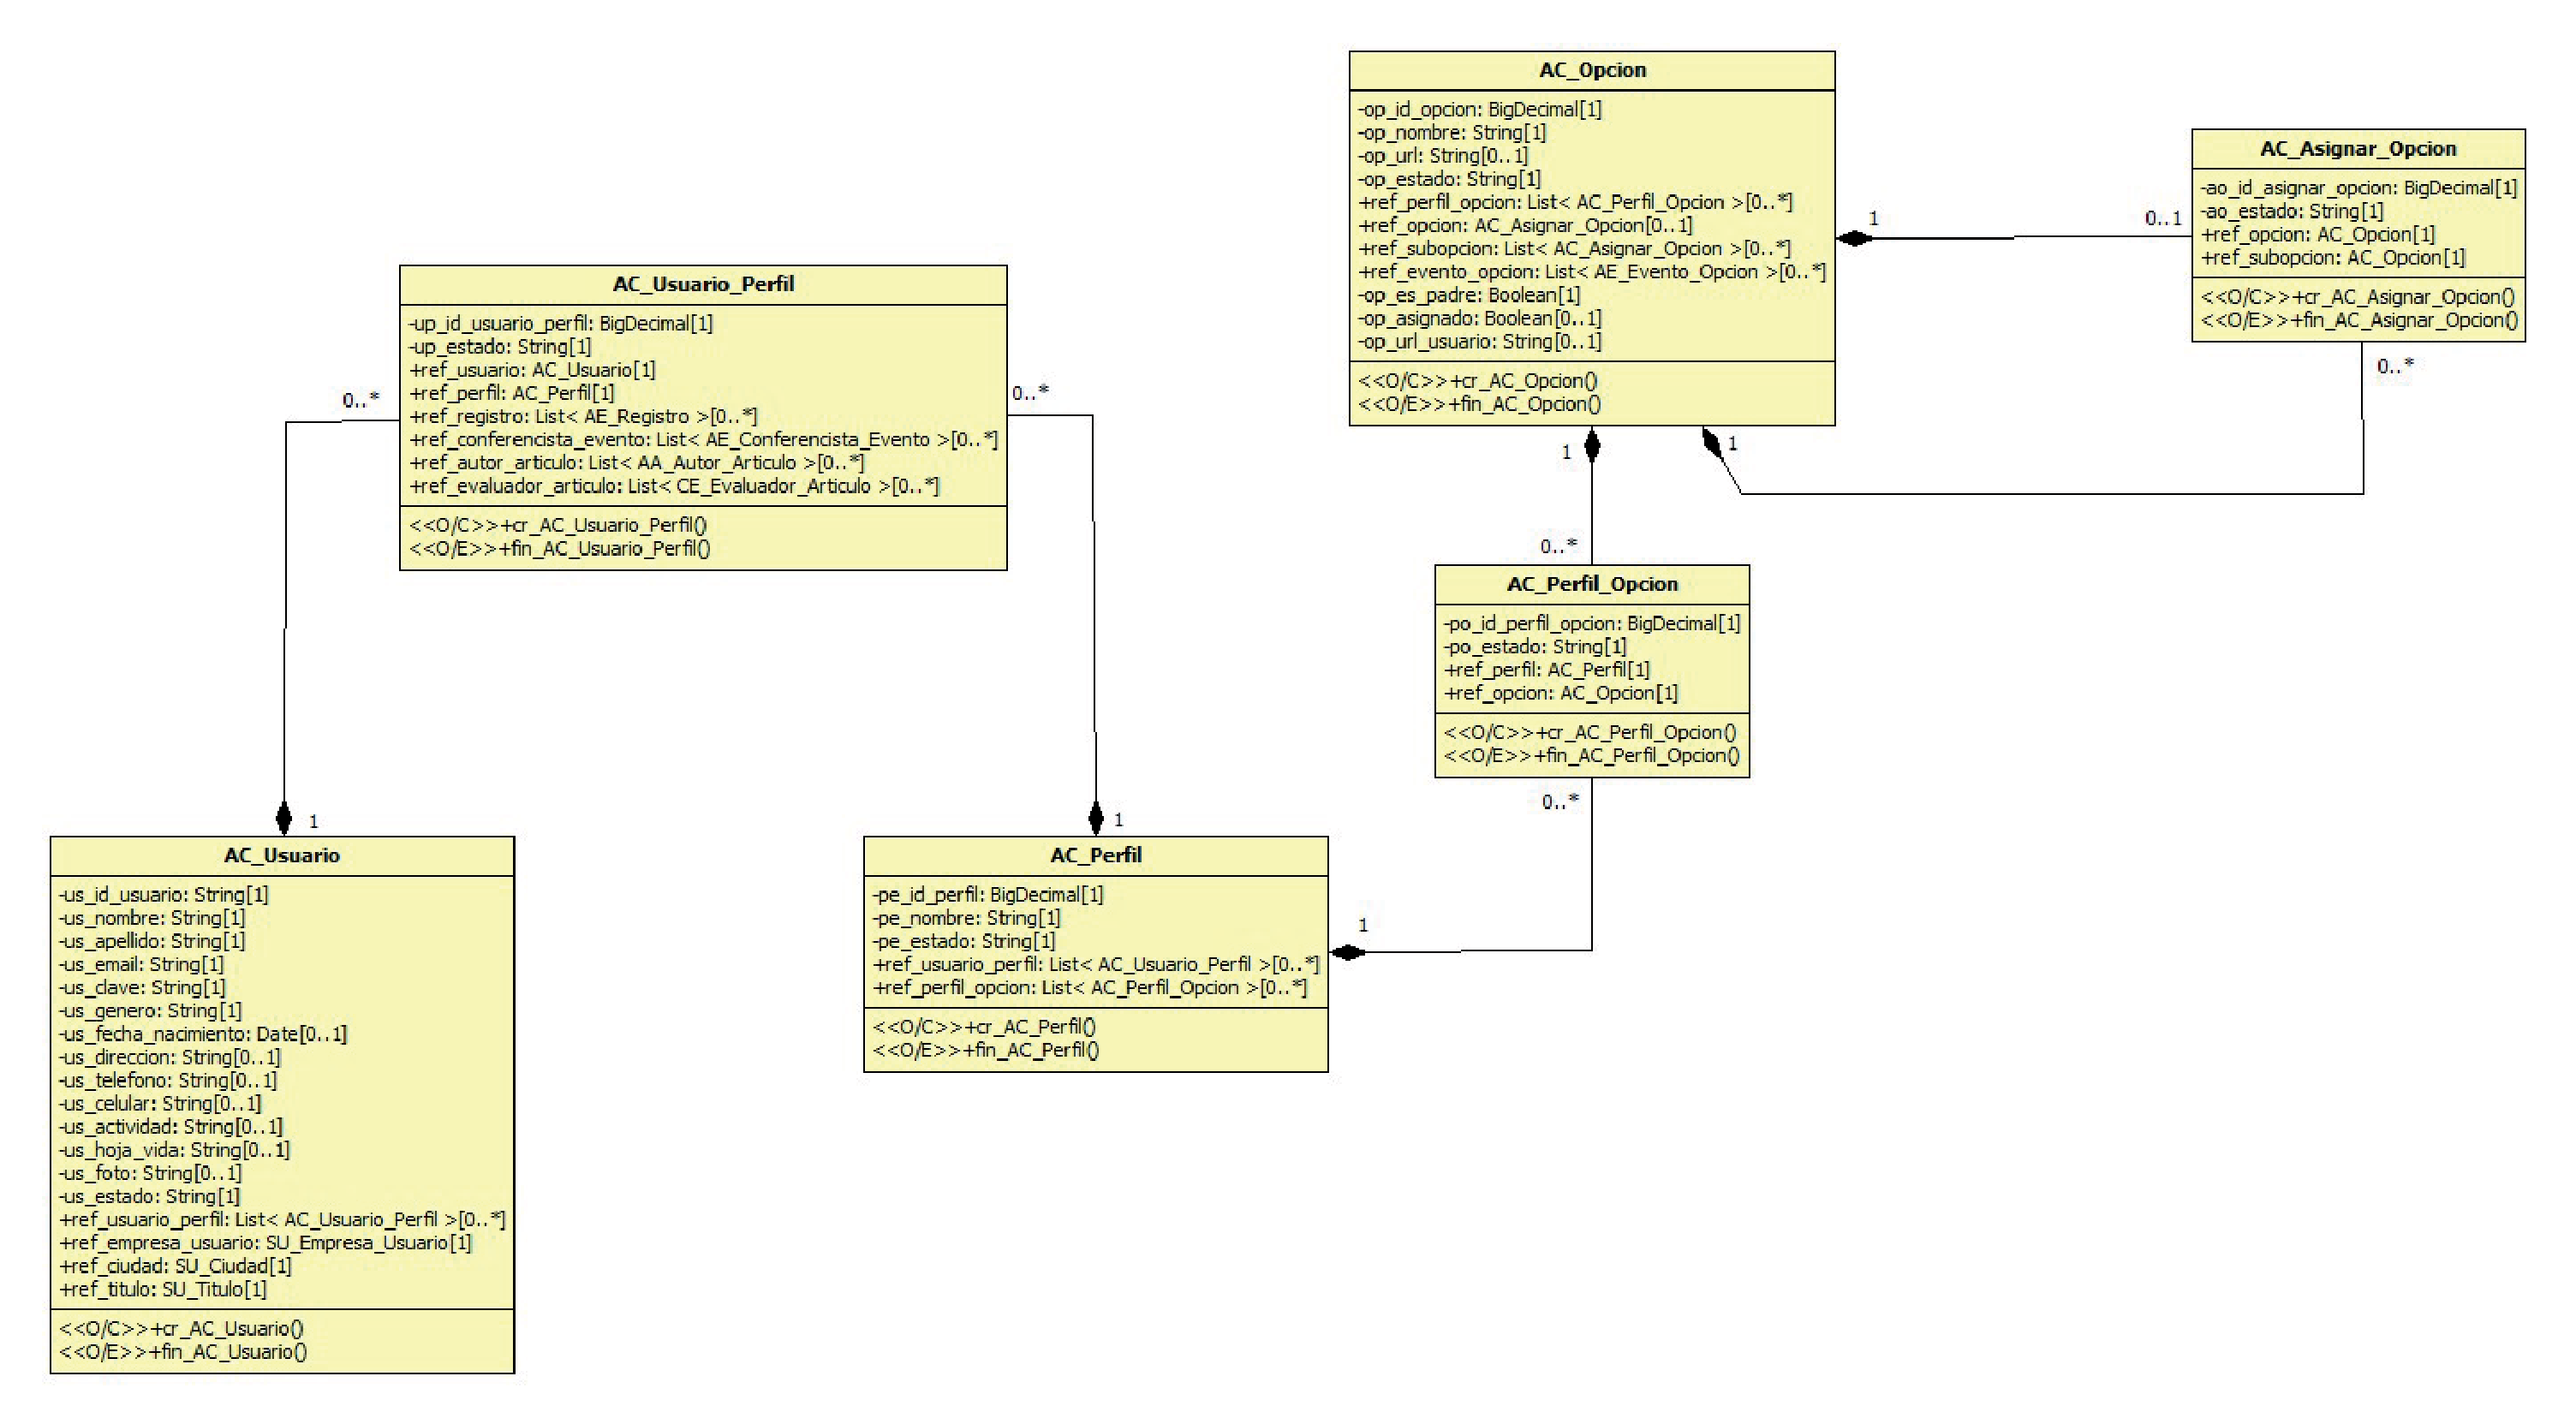
\includegraphics[width=1.7\textwidth]{images/uml-mac.eps}}
  \caption{UML - M\'odulo de Administraci\'on Central (MAC)}
  \label{uml:mac}
\end{figure}
\end{landscape}

\begin{landscape}
\begin{figure}
  \centering
    {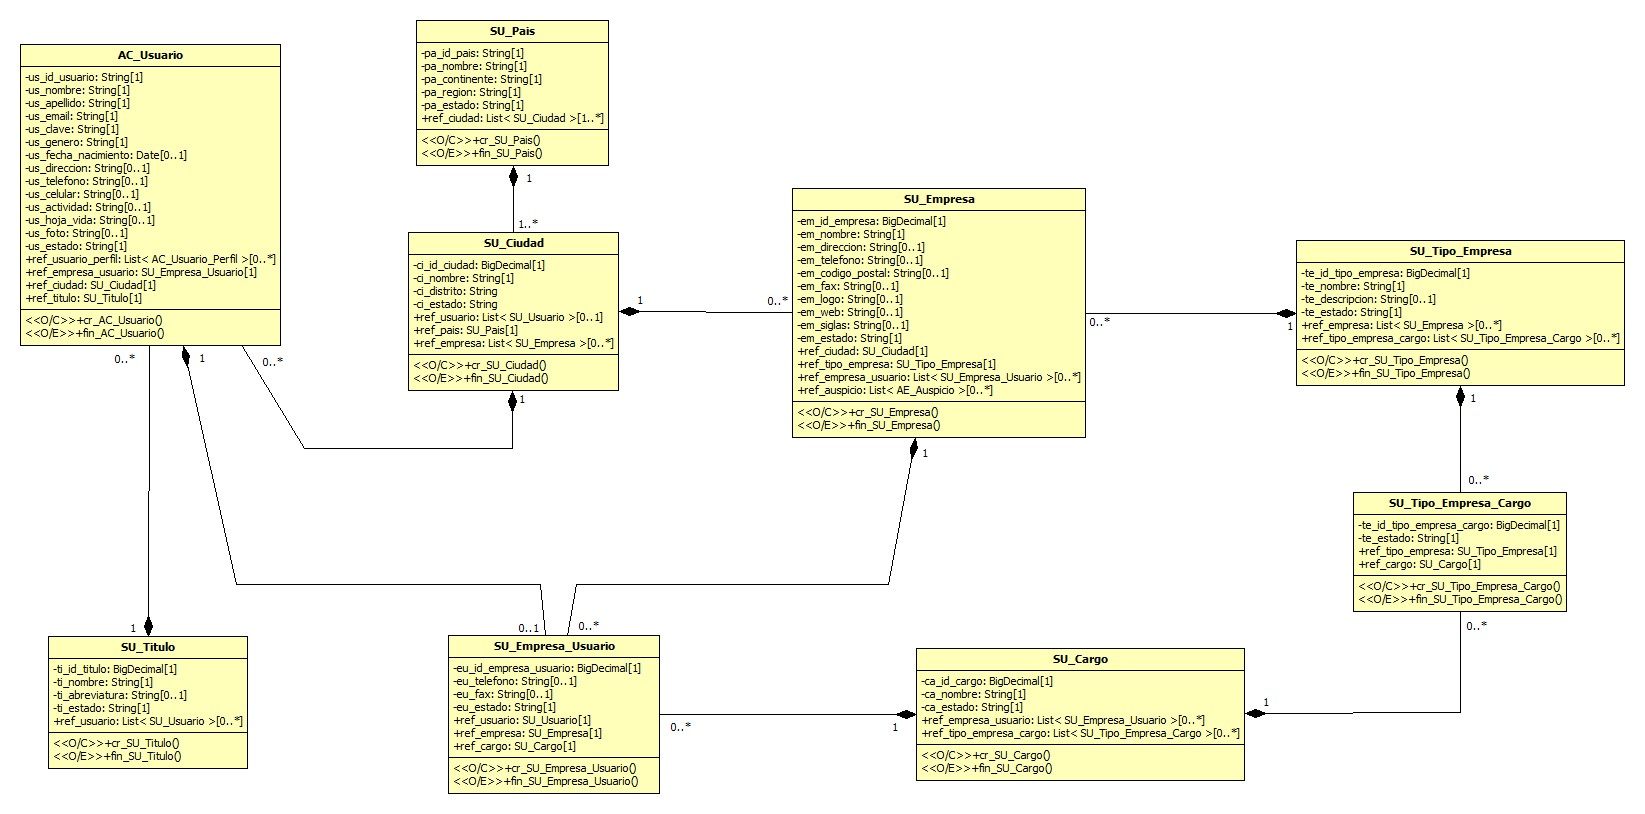
\includegraphics[width=1.7\textwidth]{images/uml-msu.eps}}
  \caption{UML - M\'odulo de Suscripci\'on de Usuarios (MSU)}
  \label{uml:msu}
\end{figure}
\end{landscape}

\begin{landscape}
\begin{figure}
  \centering
    {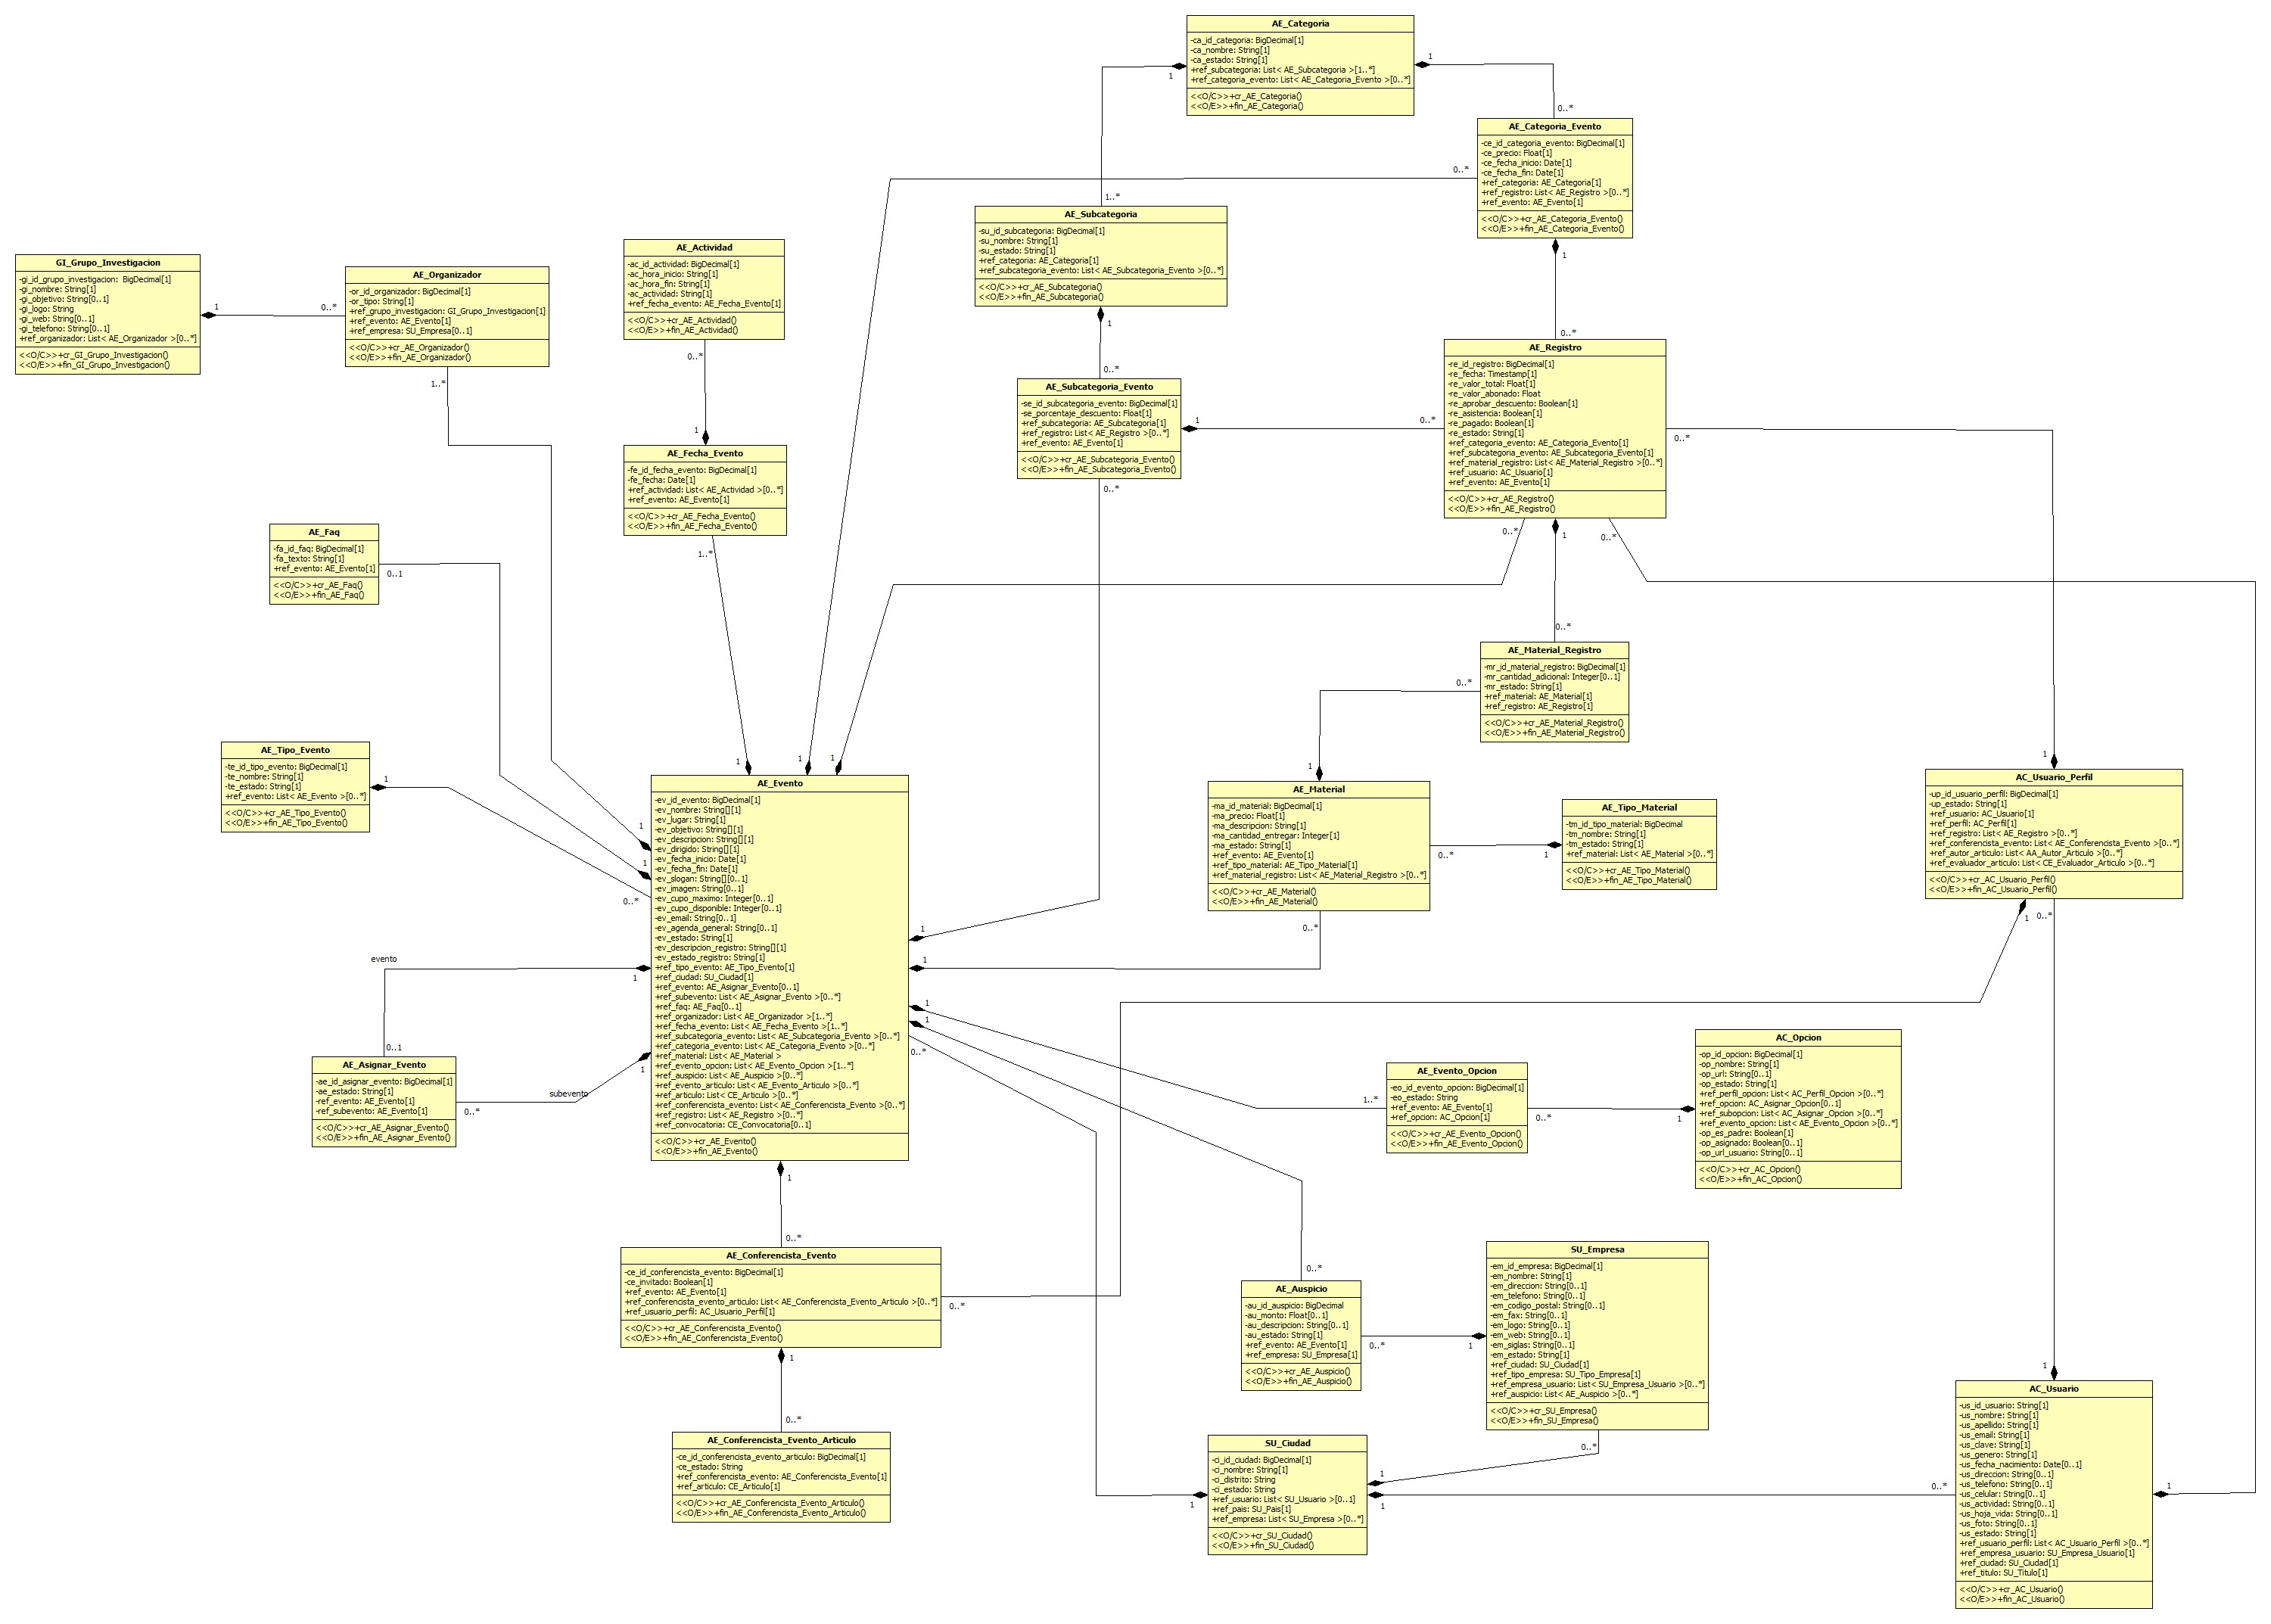
\includegraphics[width=1.3\textwidth]{images/uml-mae.eps}}
  \caption{UML - M\'odulo de Administraci\'on de Eventos (MAE)}
  \label{uml:mae}
\end{figure}
\end{landscape}

\begin{landscape}
\begin{figure}
  \centering
    {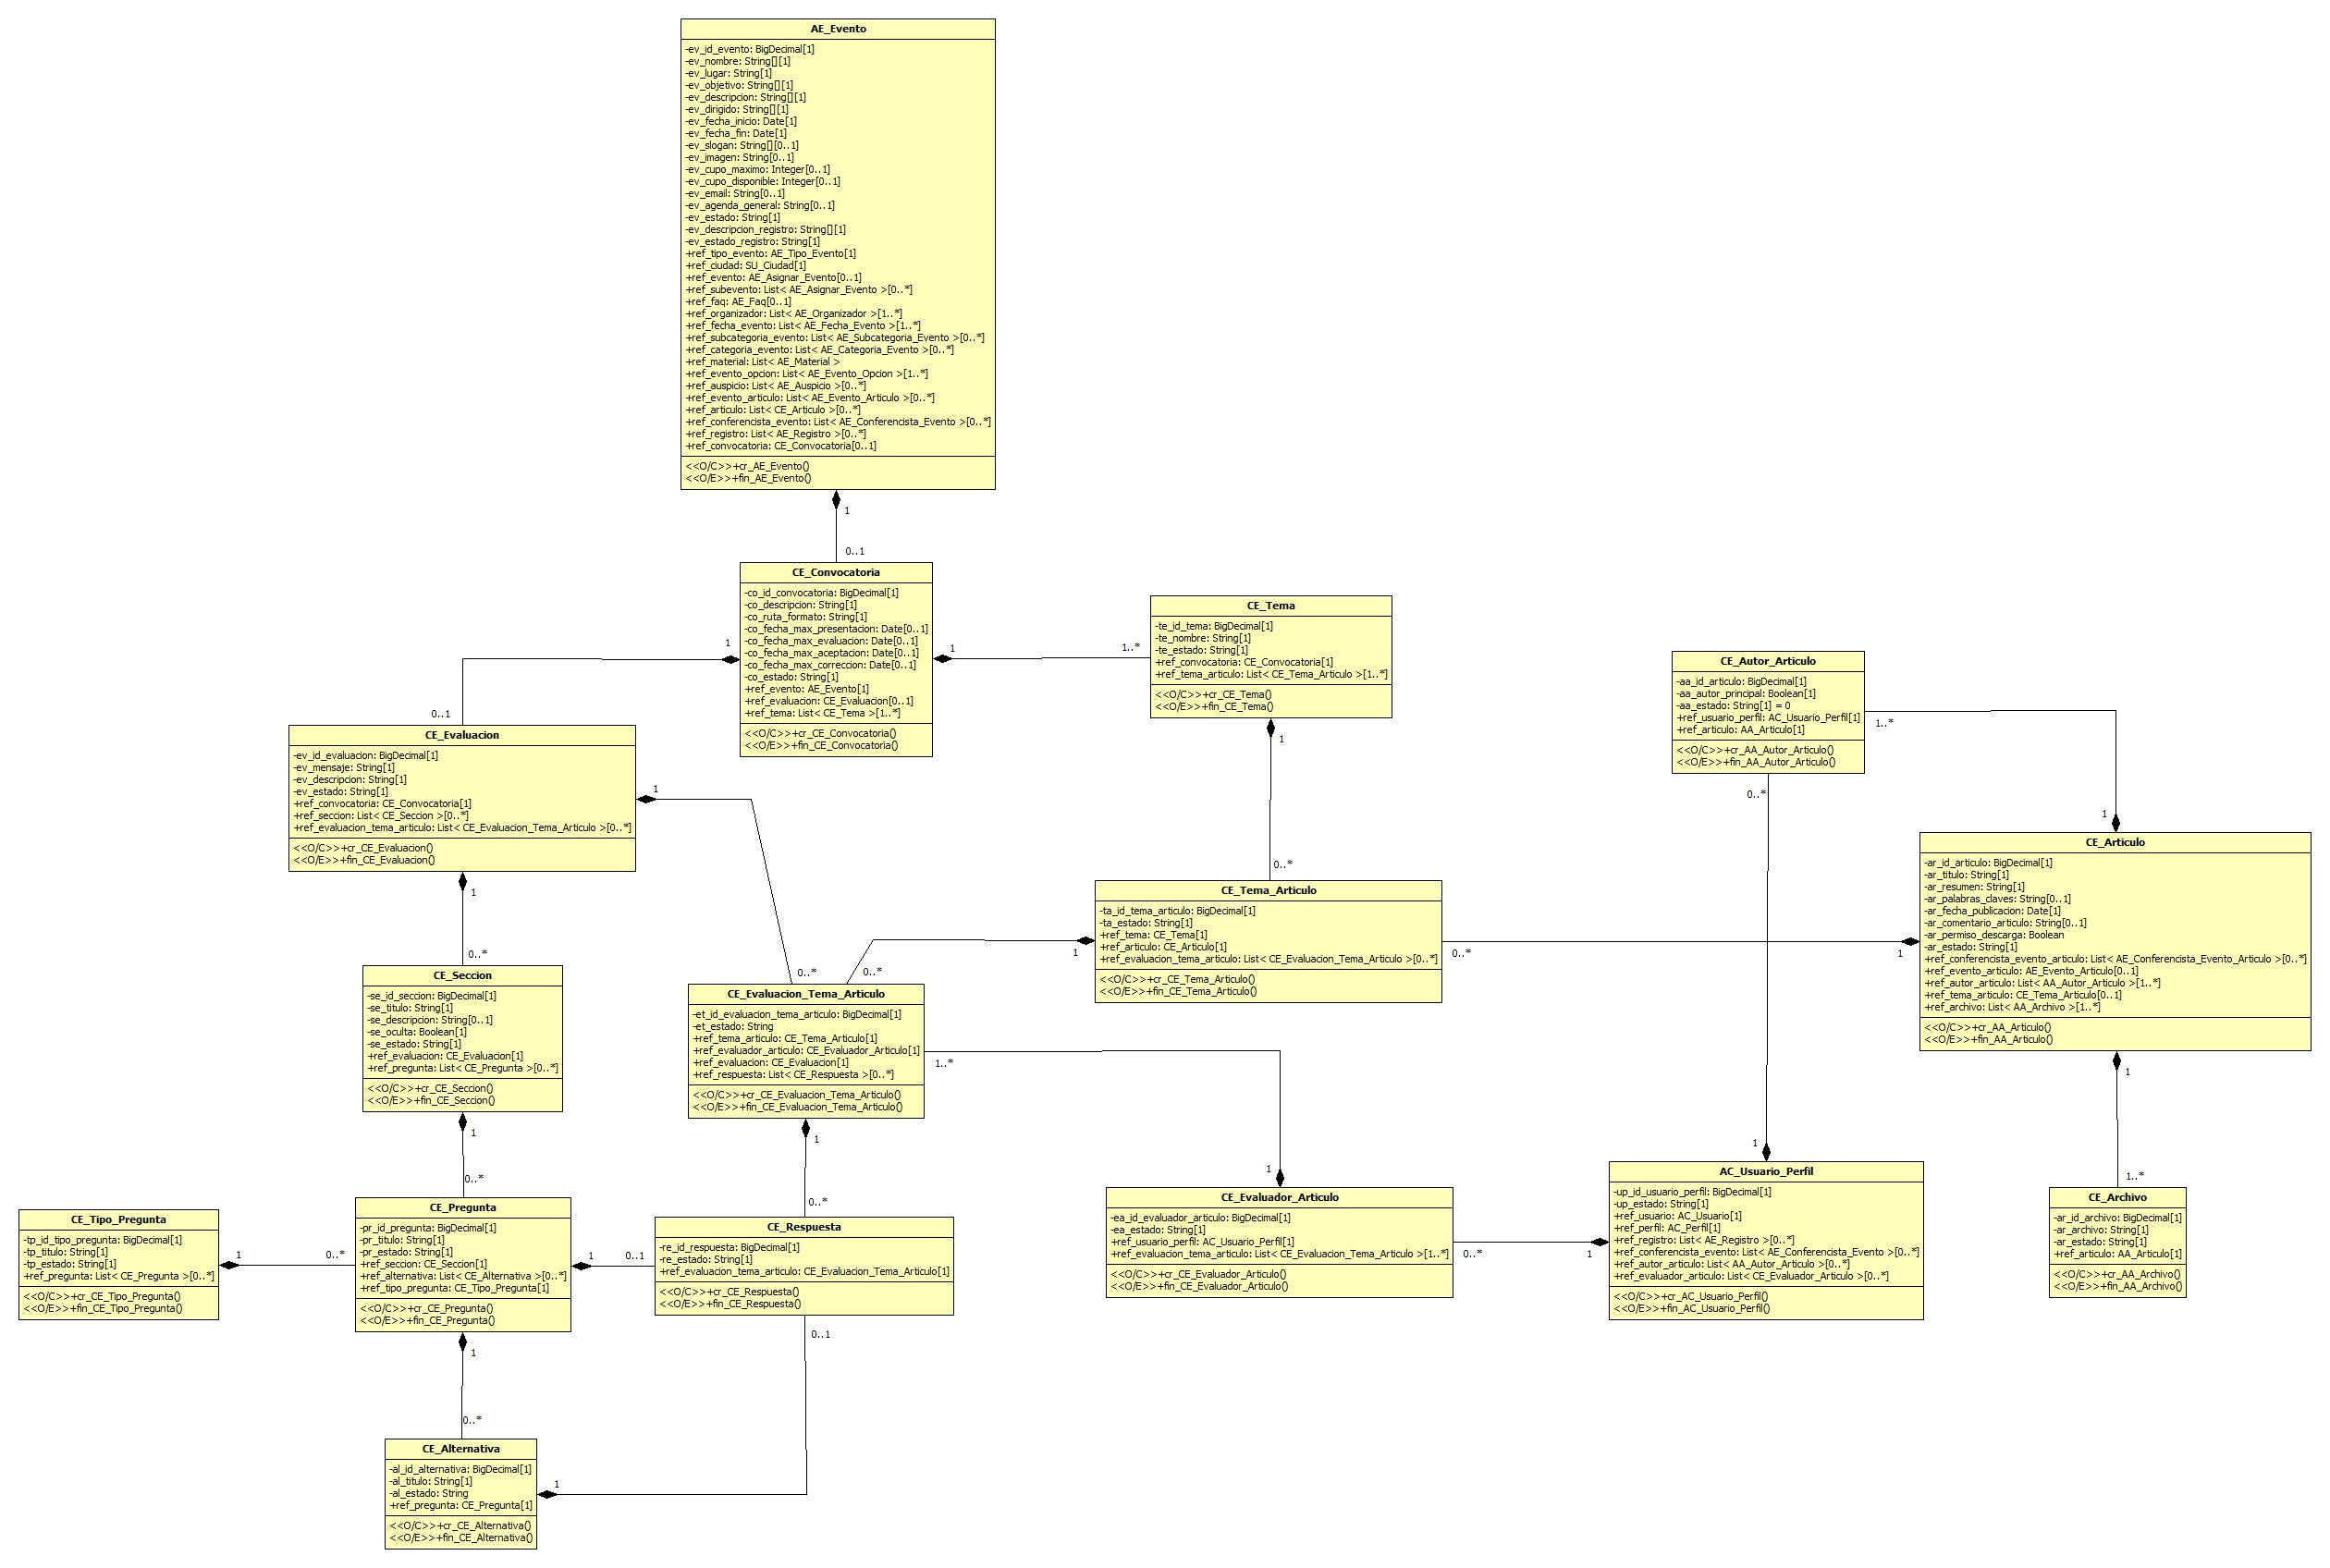
\includegraphics[width=1.5\textwidth]{images/uml-mce.eps}}
  \caption{UML - M\'odulo de Convocatoria y Evaluaci\'on de Art\'iculos (MCE)}
  \label{uml:mce}
\end{figure}
\end{landscape}

\end{indentar}

\section{Definici\'on de Roles en los M\'odulos}
\begin{indentar}
En la siguiente tabla~\ref{usuario:rol}, se muestran las funciones que ejerce cada usuario de un Grupo de Investigaci\'on desde el punto de vista de los acontecimientos del evento y desde el punto de vista del Sistema.

Cada usuario registrado en el Sistema, tiene la posibilidad de tener de uno o m\'as perfiles, de tal manera que pueden ejercer varios roles, dependiendo de las pol\'iticas especificadas por el Comit\'e Organizador.
\begin{table}
	\begin{center}
	\begin{tabular}{|p{1.5in}|p{2.2in}|p{1.5in}|}
		\hline
		\textbf{Usuario} & \textbf{Funci\'on dentro del negocio} & \textbf{Funci\'on dentro del Sistema} \\
		\hline\hline
		Director del Grupo de Investigaci\'on  	& Representante del Grupo de Investigaci\'on, encargado de planificar y elaborar las directrices para los dem\'as miembros organizadores, con la finalidad de llevar a cabo un evento de \'ambito cient\'ifico. & Administrador General \\
		\hline
		Consejo T\'ecnico Organizador		   		& Consejo conformado por los organizadores, una de sus tareas es la de decidir qu\'e resumen de un art\'iculo cient\'ifico -presentado por los posibles conferencistas- es v\'alido para darle paso al siguiente proceso de evaluaci\'on. & Administrador \\
		\hline
		Asistente del Grupo de Investigaci\'on		& Ayudante del Director del centro que sigue las directrices planificadas para la elaboraci\'on exitosa del evento.

Cabe recalcar que el asistente tiene un perfil igual al del Director, s\'olo por razones pr\'acticas. & Administrador General \\
		\hline
		Suscriptor					 						& Usuario visitante del Portal con la finalidad de estar vinculado con un Grupo de Investigaci\'on o por el deseo de registrarse a un evento.  & Suscriptor \\
		\hline
		Evaluador											& Participante del evento en calidad de evaluador, con el prop\'osito de verificar la utilidad del conocimiento demostrado en el art\'iculo. & Evaluador \\
		\hline
		Conferencista										& Usuario que present\'o un art\'iculo de \'indole cient\'ifico con un resultado exitoso, el conferencista tambi\'en puede ser invitado por el Comit\'e Organizador. & Conferencista \\
		\hline
	\end{tabular}
	\caption{Definici\'on de Roles en los M\'odulos}\label{usuario:rol}
	\end{center}
\end{table}
\end{indentar}
